\documentclass[a4paper, 12pt]{article}

% Set margins
\usepackage[hmargin=2cm, vmargin=2cm]{geometry}

\frenchspacing

% Language packages
\usepackage[utf8]{inputenc}
\usepackage[T1]{fontenc}
\usepackage[magyar]{babel}

% AMS
\usepackage{amssymb,amsmath}

% Graphic packages
\usepackage{graphicx}

% Colors
\usepackage{color}
\usepackage[usenames,dvipsnames]{xcolor}

% Enumeration
\usepackage{enumitem}

\title{Architektúrák, beágyazott rendszerek (GEVAU218M)\\\LARGE{\textbf{Beszámoló}}\\ \bigskip \Large{\textit{LED mátrix kijelzős óra és szöveg scroller}}}
\date{2020. november 21.}
\author{Nagy Dániel Zoltán JJ181J}

\begin{document}

\maketitle

\section{Leírás}
A féléves beadandó feladatomnak egy óra elkészítését választottam.
Az eszköz egy LED mátrix kijelzőn a pontos időt mutatja. A kijelzőn minden harmincadik másodpercben csúszó szövegkként megjelenik a napi dátum és az aktuális napnak a neve. A felhasználónak lehetősége van szöveget küldeni az eszköznek. Ezt az eszköz által szolgáltatott weboldalon teheti meg. A szöveg a kijelzőn annyiszor csúszik végig amennyiszer azt a felhasználó beállította. A weboldalon lehetőségünk van a kijelző fényerejét is konfigurálni.

\begin{figure}[ht]
	\centering
	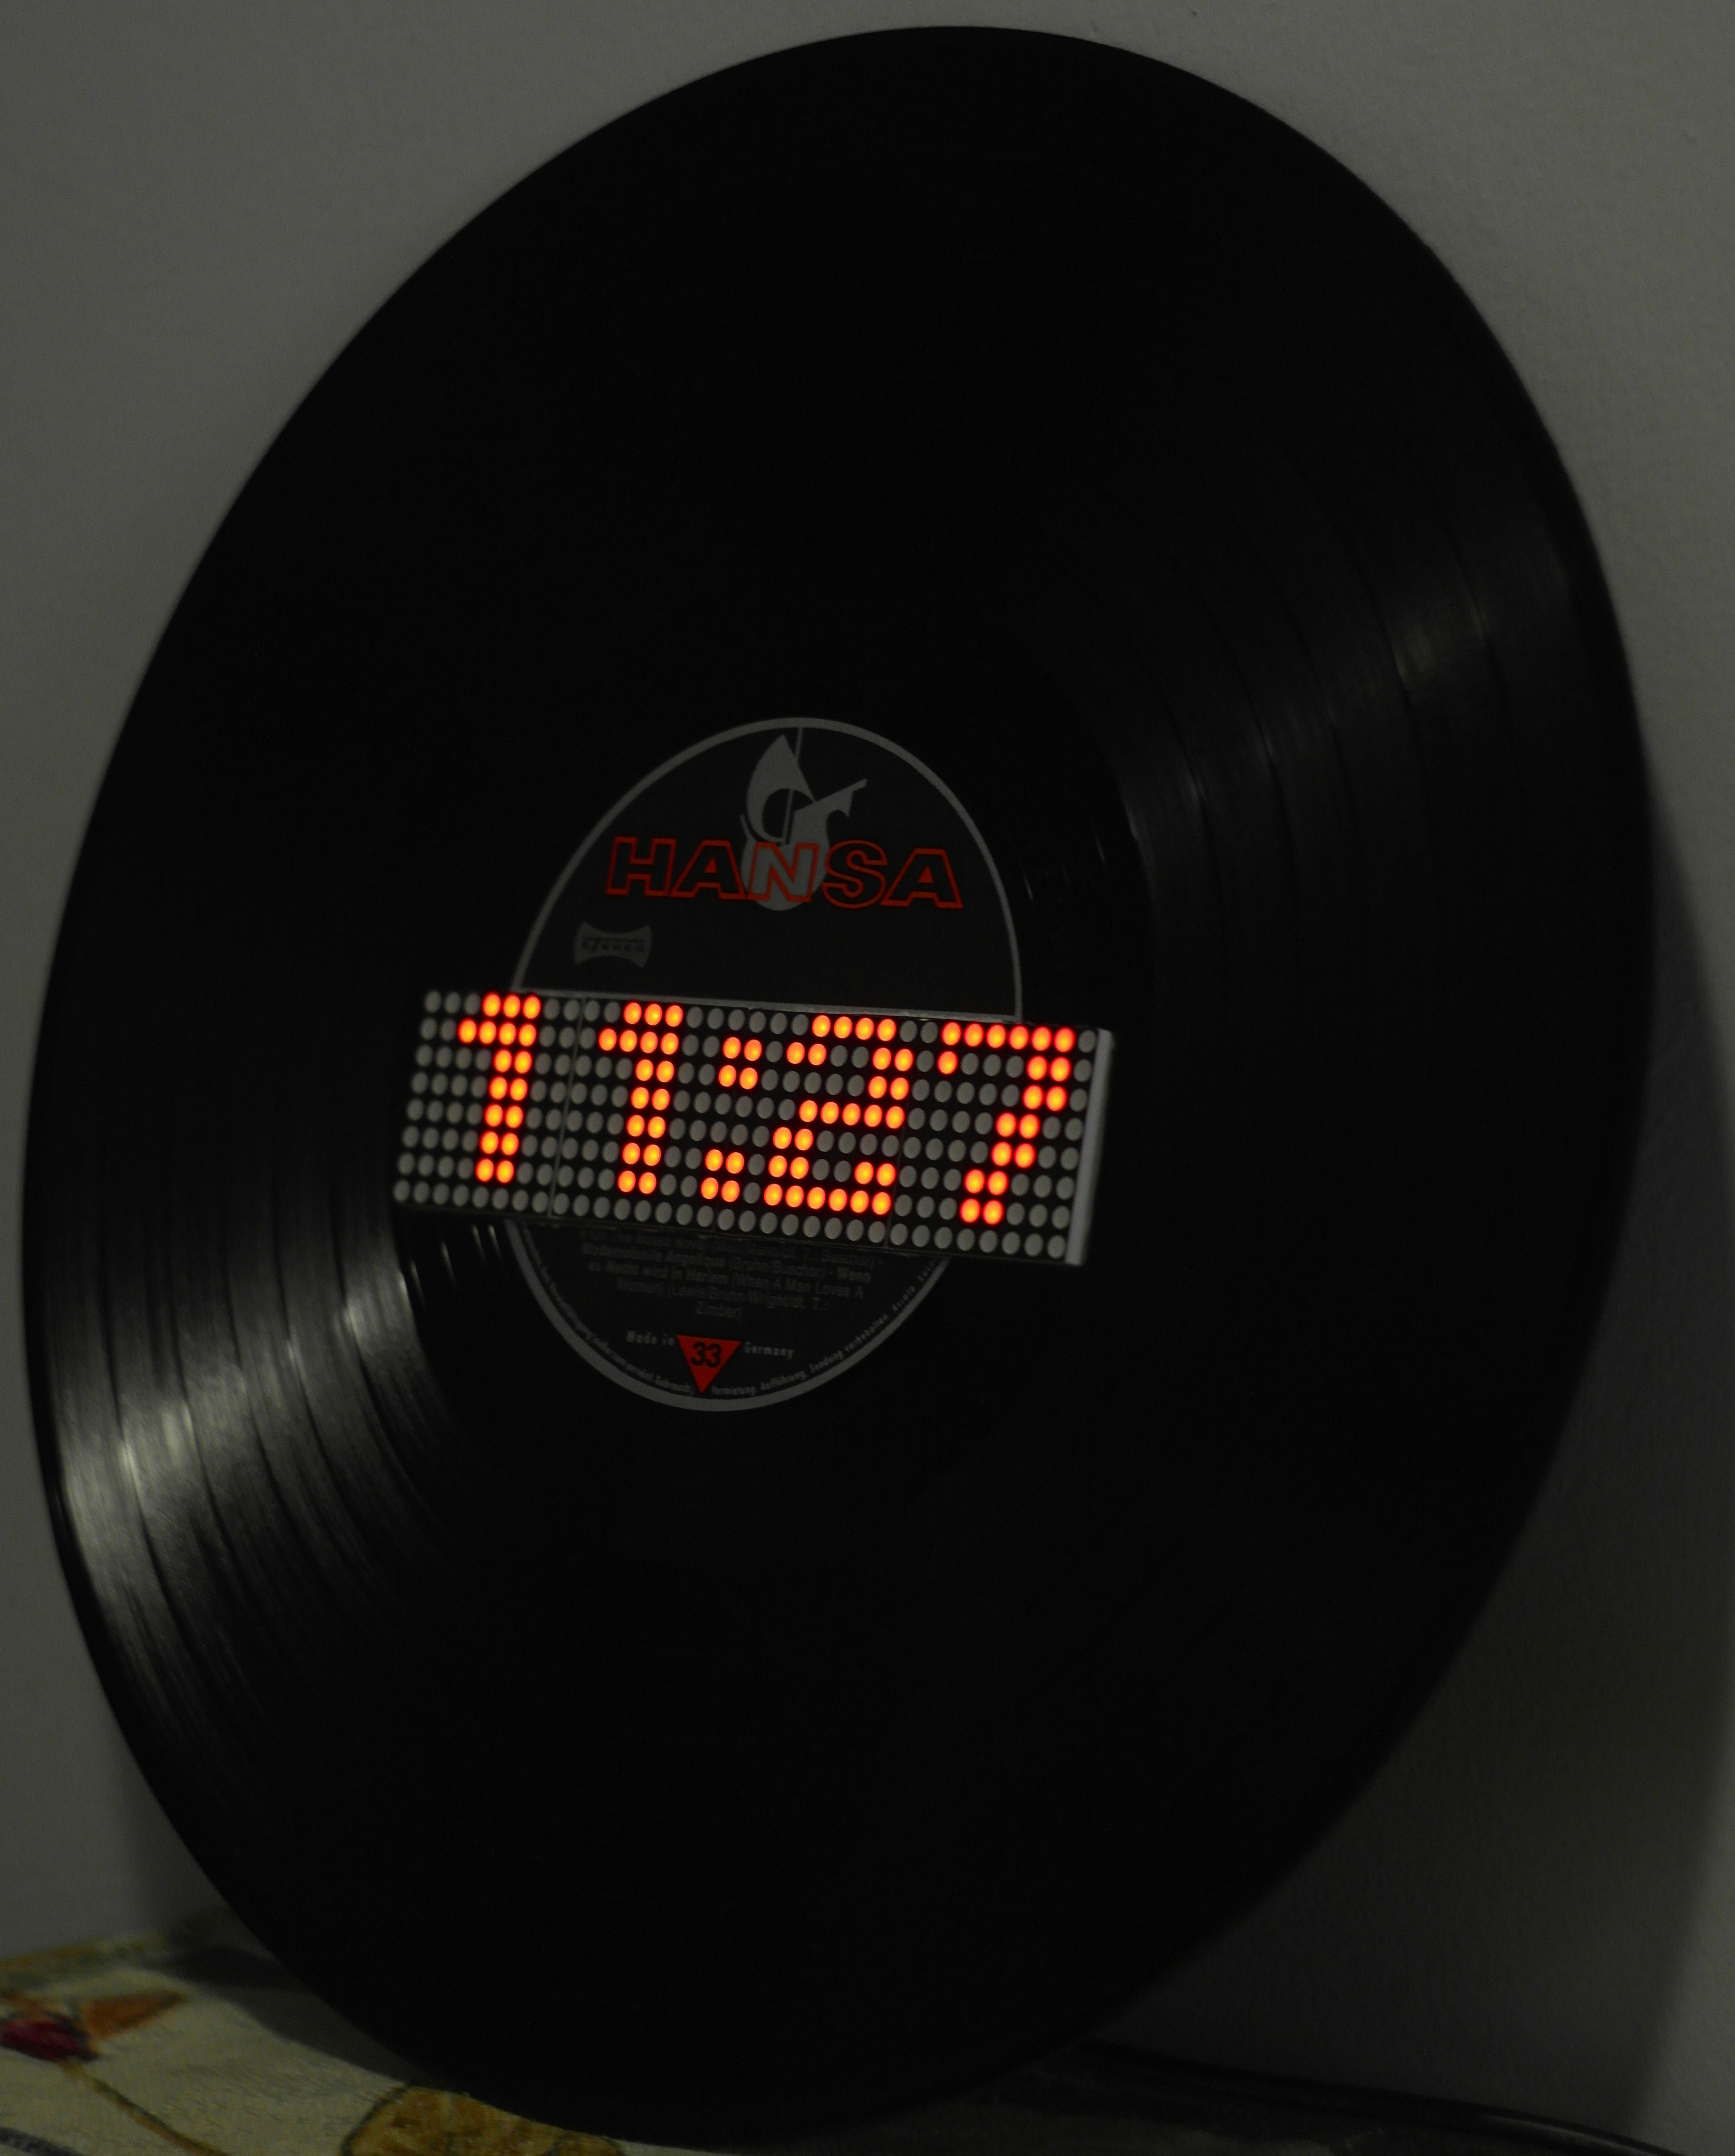
\includegraphics[width = 9cm]{images/vinyl_clock.JPG}
	\caption{Fénykép az elkészült feladatról}
	\label{fig:product}
\end{figure}	

\section{Működés}

\subsection{Megjelenítés}
Az eszköz egy mátrix kijelzőn jeleníti meg a kiírandó tartalmakat. A kijelző cellái különálló $8\times 8$-as LED mátrixok. Az egymás után fűzött cellák alkotják a kijelző felületét. A feladatomhoz 4 db cella elegendő, hiszen akkora felület tökéletesen alkalmas egy digitális óra 4 számjegyének megjelenítésére, és a csúsztatott szöveg kijelzése is megoldható vele, hiszen a 4 mátrix megfelelő szélességű felületet biztosít a szavak olasható kirajzolásához.

A szövegek megjelenítése érdekében szükséges a mátrixon megjeleníthető karakterek definiálása. Az egyes karakterek képe leírható egy bináris kétdimenziós mátrix formájában, ahol az 1 érték világító, a 0 pedig kikapcsolt LED-et jelöl.
A karakterek dimenzióját a mátrix méretei határozzák meg. Vagyis a karaterek maximum mátrix mérete is $8\times 8$-as lehet. A magasság minden esetben 8 egy, a szélesség viszont változó lehet. A változó karakterszélesség használatával a szavak egybefüggőbbnek látszanak.

Példa egy G betű képére:
\begin{center}
\textbf{0 1 1 1 0\\
1 0 0 0 0\\
1 0 0 0 0\\
1 0 0 1 1\\
1 0 0 0 1\\
1 0 0 0 1\\
0 1 1 1 0\\
0 0 0 0 0}
\end{center}
A fenti példából látható, hogy a betű képét egy $5\times 8$-as bináris mátrixxal írhatjuk le. A karaktereket állítva rajzoltam meg. A legalsó sor a legtöbb esetben üres, így a betűk maximum 7 egység magasak.

\begin{figure}[ht]
	\centering
	\includegraphics[width = 10cm]{images/hetfo.JPG}
	\caption{Hétfő - csúszás közben}
	\label{fig:hetfo}
\end{figure}	


A karakterek azonosítása az ASCII karakterkódjaik alapján történik. Mivel nem definiáltam a teljes ASCII karakterkészletet, így bizonyos esetekben az üres helyek miatt ki kell vonni a karakterkódból a kihagyott karakterszám értékét, hogy megkapjuk a keresett karakter képének az indexét.
Ha a soron következő karakter ASCII kódja 32 és 90 közé esik, akkor 32-t kell levonni. Ha pedig 97 és 122 közé esik, akkor 38-at. A nem definiált karakterek helyett egy * képét illeszti.
Az ékezetes karakterek már nem alkotnak egybefüggő területet az ASCII kódtáblában, így hivatkozásuk egyedi értékek szerint történik.

A képernyőn megjelenő tartalom szintén egy kétdimenziós bináris mátrixalakban írható le. Méretei az egymás után összefűzött cellák által adott felületéből adódnak. Egy 4 cellából álló kijelző esetében a kijelző mérete: $32\times 8$.
A megjelenítéshez ezt a nagy mátrixot kell manipulálnunk.

\subsubsection{Csúszó szöveg}
A csúszó szöveg megjelenítése a következő képpen tehető meg:
Vegyünk egy $n$ karakterből álló szöveget és legyen két mutatónk: $i$, ami a soron következő karakterre mutat és $j$, amely az aktuális karakter mátrix alakjának az oszlopaira mutat. $i = 0$, $j = 0$.
A szöveget a képernyő jobboldaláról csúsztatjuk balra.
\begin{enumerate}
	\item Vegyük az szöveg $i$-edik karakterét.
	\item Az $i$-edik karakter $j$-edik oszlopát helyezzük a mátrix utolsó oszlopába.
	\item A mátrixot egy egységgel toljuk el balra. Az első oszlopa így törlődik, a jobb szélére helyezzünk egy üres oszlopot.
	\item A mátrix képét jelenítsük meg a kijelzőn, majd várjunk $t$ időegységnyit.
	\item Növeljük a $j$ értékét eggyel, majd térjünk vissza a 2. lépésre. Egészen addig ismételjük, amíg a $j \leq$ az $i$-edik karakter képének szélességével.
	\item A mátrixot egy egységgel toljuk el balra a már ismert módon, hogy a karakterek között egy üres oszlopot hagyjunk.
	\item Növeljük az $i$ értékét eggyel, majd térjünk vissza az 1. lépésre. Egészen addig ismételjük, amíg $i \leq n$.
\end{enumerate}

A fenti eljárásban a $t$ értéke tetszőleges lehet. Minél kisebb a várakozási idő, annál gyorsabban fog a kiírandó szöveg csúszni a képernyőn.

\subsubsection{Az óra számlapja}

\begin{figure}[ht]
	\centering
	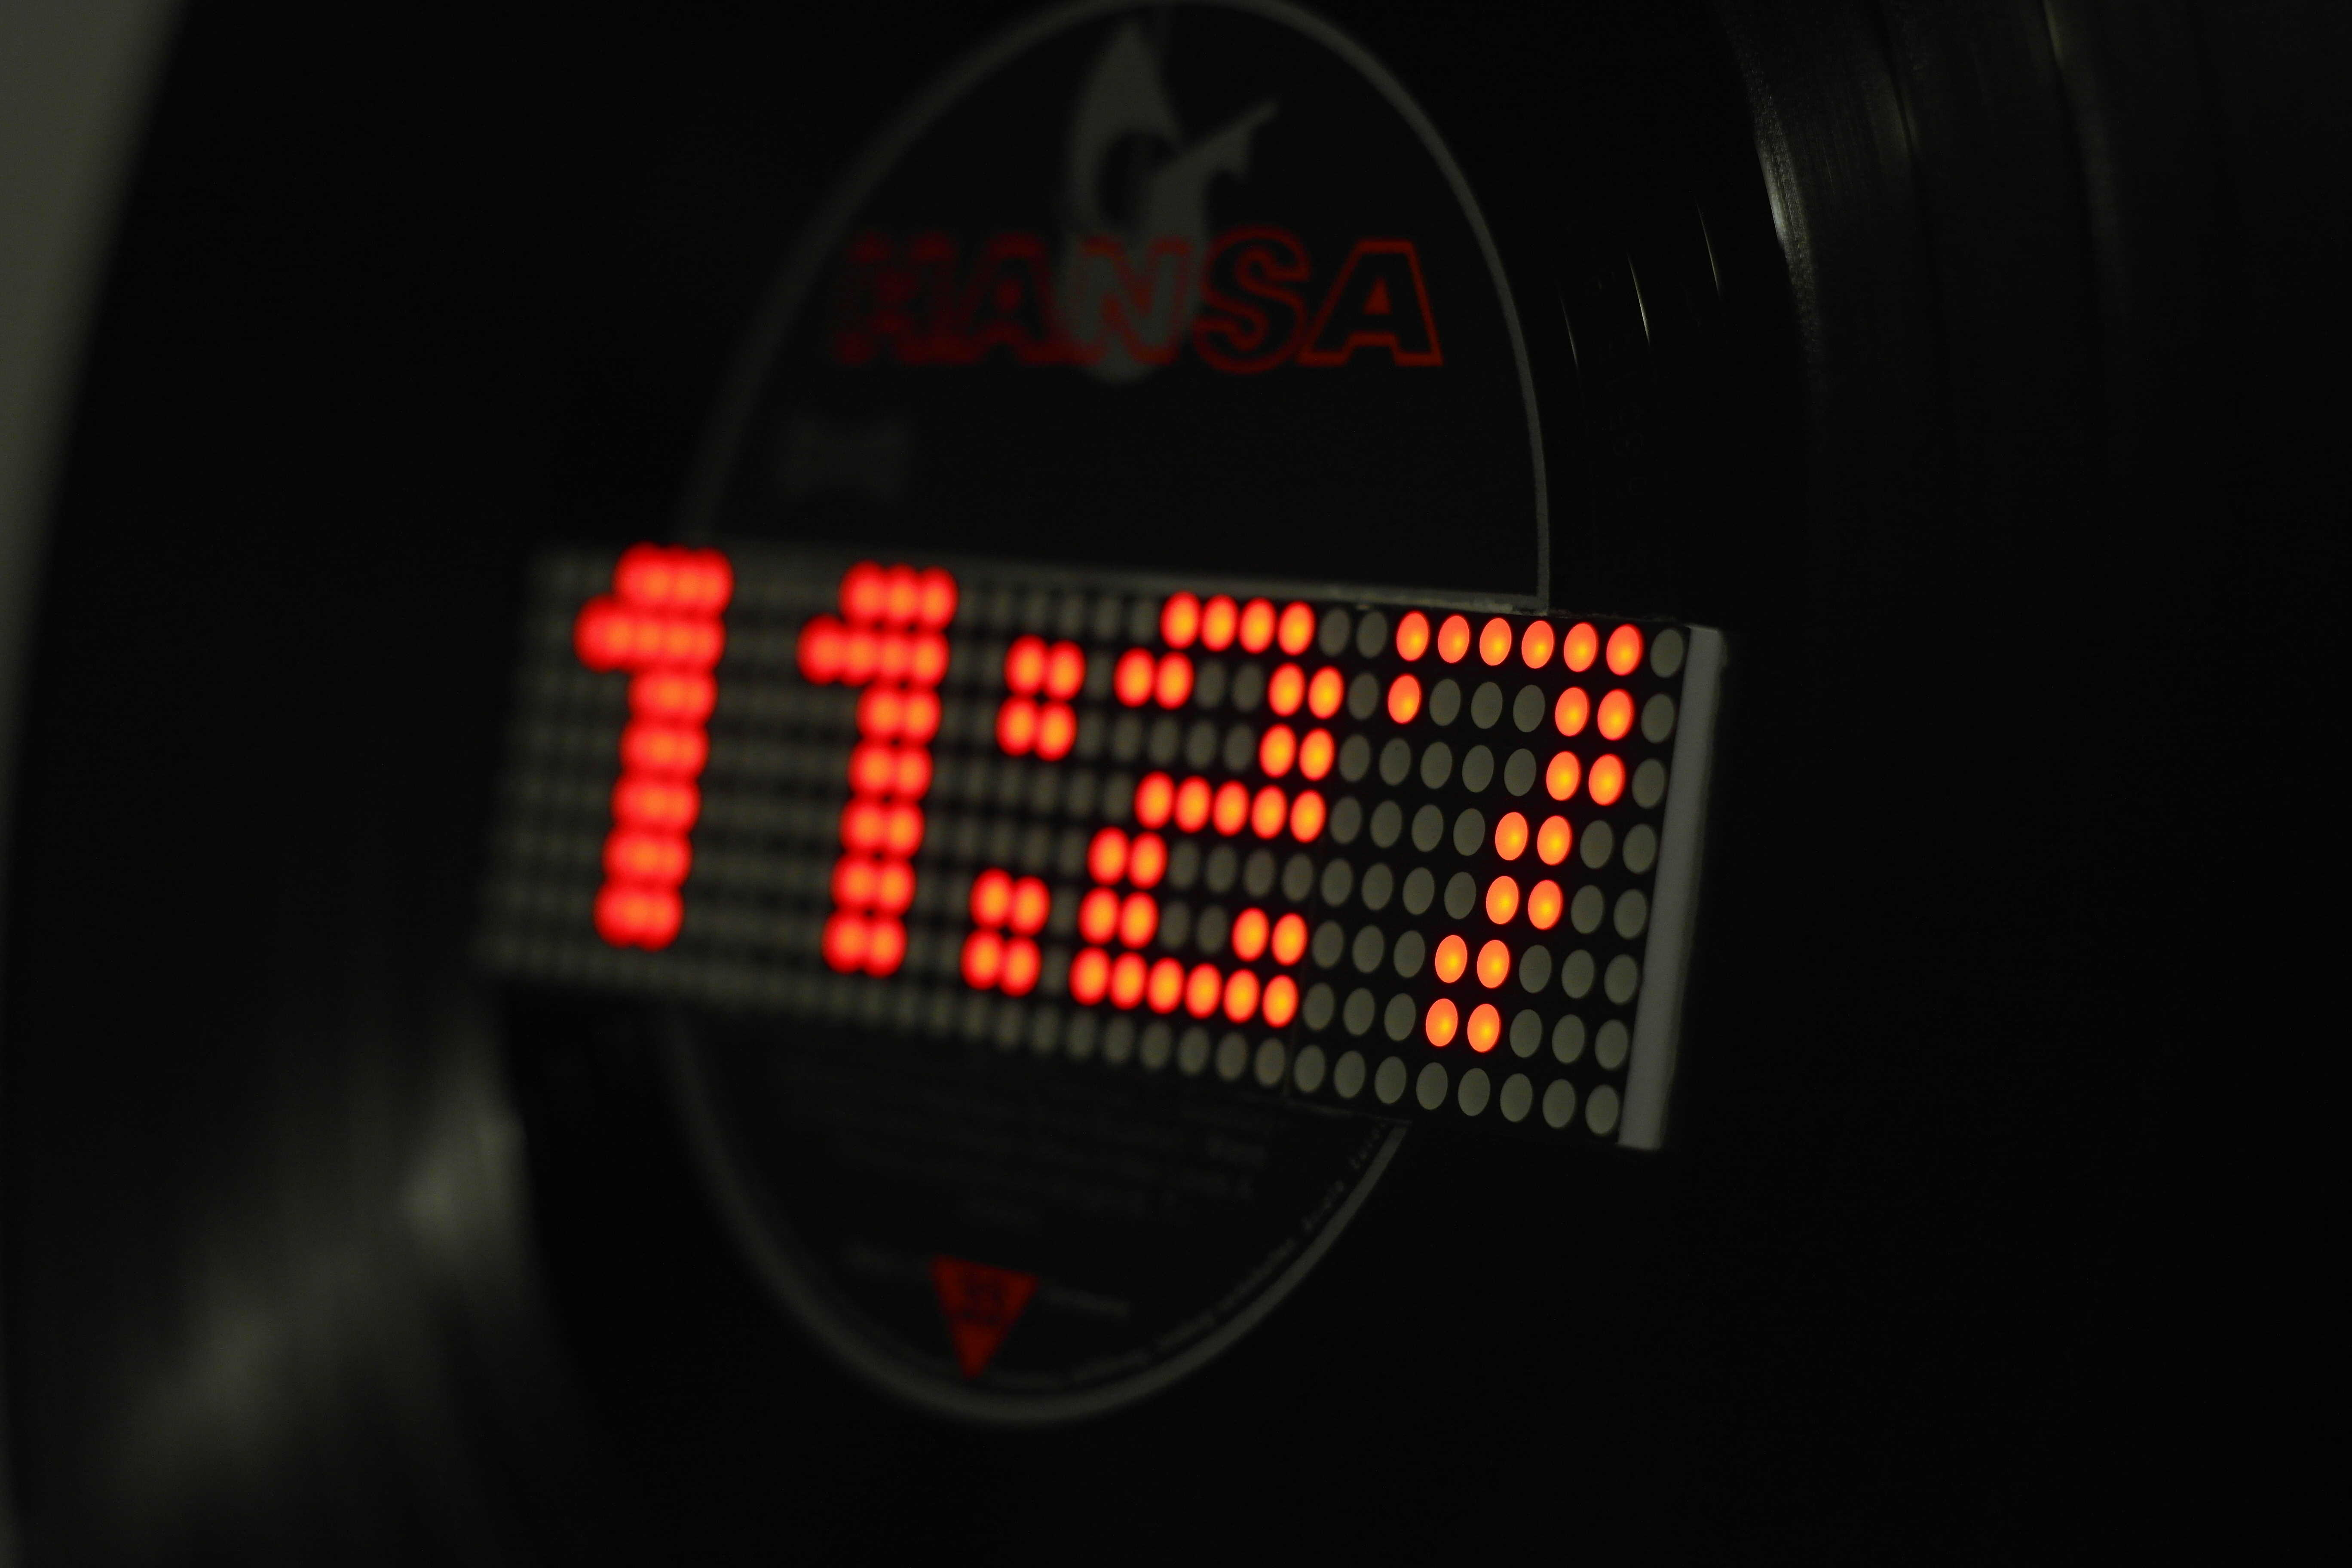
\includegraphics[width = 10cm]{images/clockface.JPG}
	\caption{Fénykép az óra számlapjáról}
	\label{fig:clockface}
\end{figure}	

Az óra számlapjának megjelenítéséhez szintén a kijelzőt reprezentáló mátrixot manipuláljuk.
Ebben az esetben fix pozíciókat használunk és a megjelenítendő számjegyek mátrixképei azonos szélességűek.
Az óra számjegyeihez egy külön karakterkészletet definiáltam, amelyek 0-9 reprezentálják a számokat. Ennek csupán esztétikai jelentősége van, a számjegyek a már meglévő karakterektől vastagabbak.
Az óra számlapja 4 számjegyből áll és a középen elhelyezkedő kettőspontból.
A 10-nél kissebb számjegyek elég egy nullást illesztünk, hogy a megjelenített kép szimmetrikus legyen.

\subsection{Vezetéknélküli kommunikáció}
Az eszközön megjelenő szöveget saját hálózaton keresztül van lehetőségünk küldeni. Az eszköznek csatlakoznia kell a felhasználó hálózatára. Ezt WIFI kommunikációs protokollon valósul meg. A csatlakozást követően az eszköz a routertől kap egy saját IP címet és a 80-as portján egy HTTP szervert szolgáltat.
A szerveralkalmazás rendkívül egyszerű. Két kérést vesz vigyelembe: a GET, illetve a POST kéréseket.
Ezen kérések aszinkron léphetnek fel. Így a kérések beérkezésekor az üzenetet el kell tárolnunk egy \textit{bufferben}. Ha az ütemező a szervernek adja a futási jogot, az a már a buffer tartalmát dolgozza fel.
A programomban egyetlen buffert használok. Ez problémát jelentene akkor, ha egyszerre több kérés érkezne be. Ilyenkor szerencsésebb lenne egy ún. körkörös buffer használata. De mivel az eszköz otthoni használatra lett tervezve, amelynek hálózatán kevés kliens van jelen, így egy buffer is elegendő a feladathoz.

\begin{figure}[ht]
	\centering
	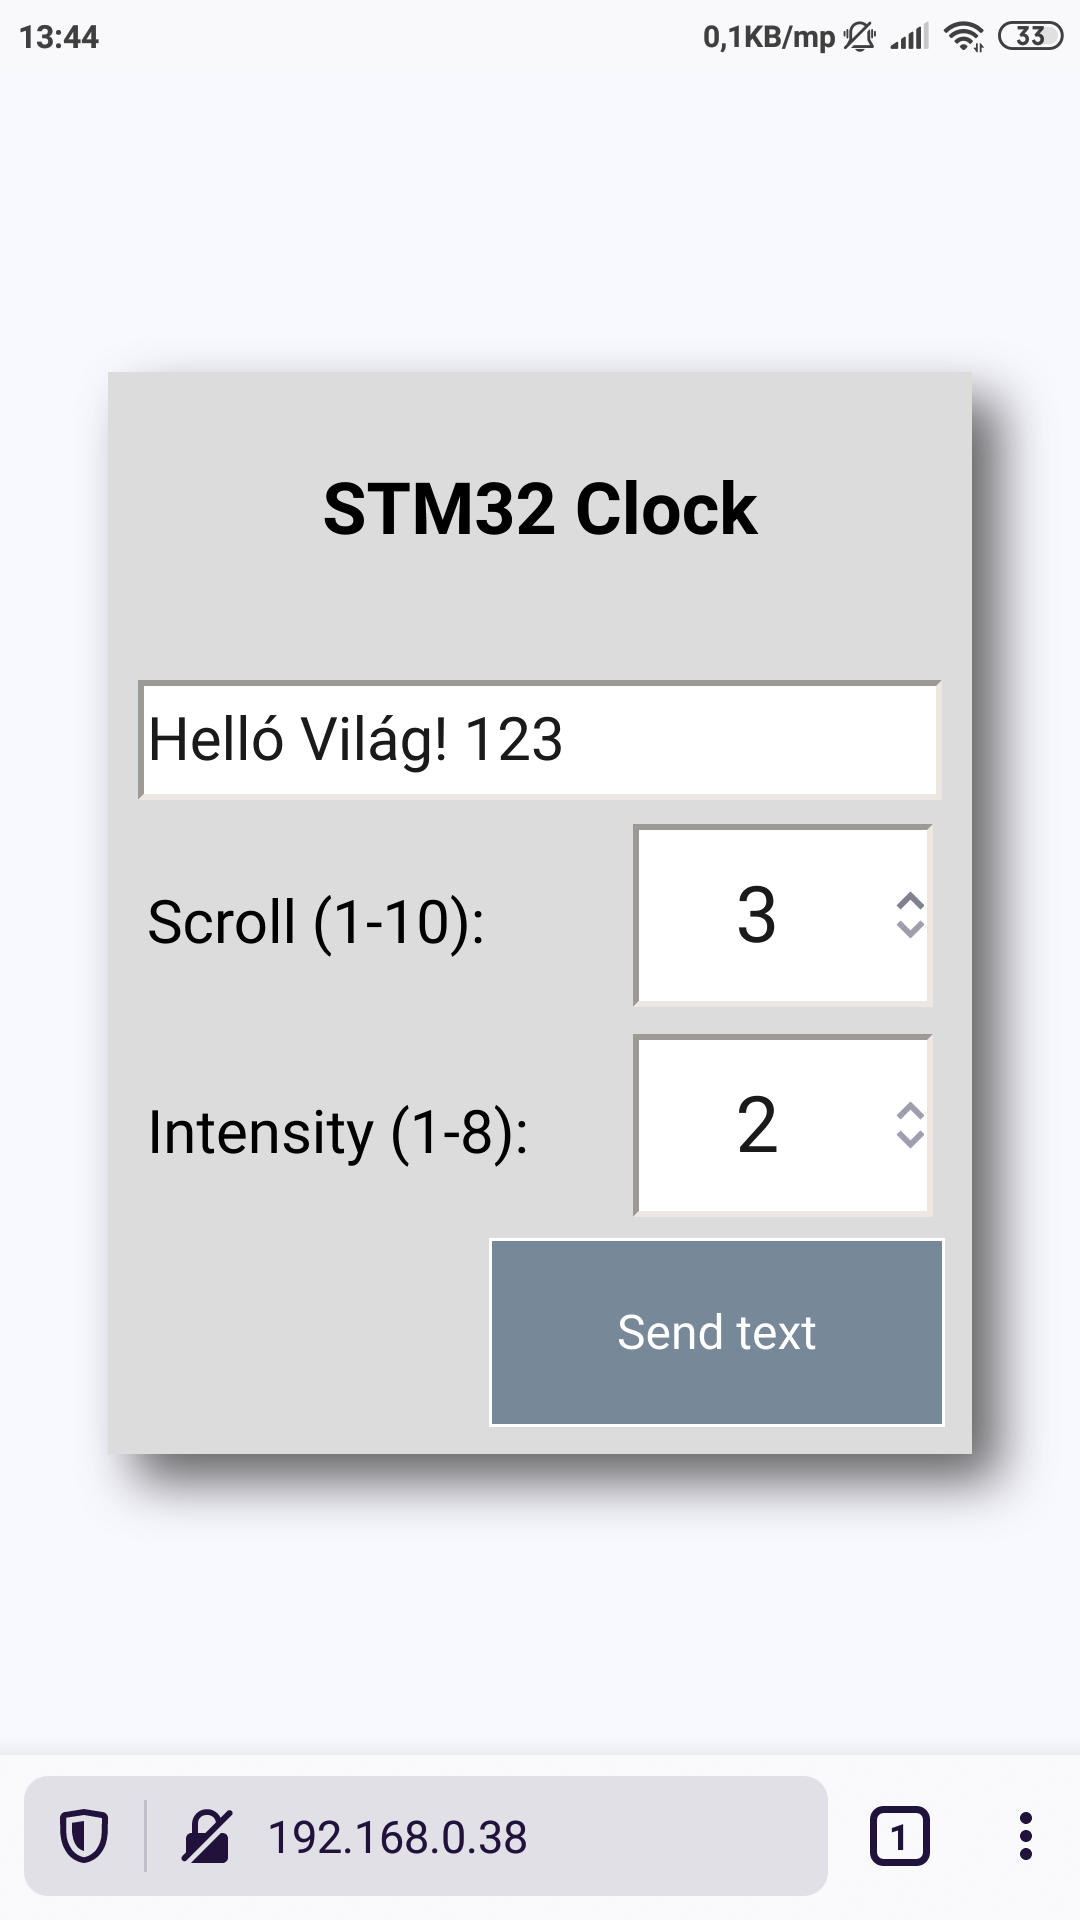
\includegraphics[width = 7cm]{images/webpage.png}
	\caption{Képernyőfotó a weblapról (\textit{Mozzilla böngésző, Android})}
	\label{fig:webpage}
\end{figure}	

\subsubsection{GET}

GET kérés esetén feltételezhetjük, hogy a kérés a weboldal betöltésére irányul, egy böngészőablakból. A kéréshez minden esetben tartozik egy \textit{link ID} is, vagyis egy azonosító, amely a kiszolgálásra váró klienseket jelöli. A kérés beérkezésekor az eszköz kiküldi a weboldalt a kliensnek. A weboldal tartalma egy inputmező, amleyben a kliensek szöveget írhatnak. Az inputmező alatt a kliens megadhatja, hogy a szövege hányszor csússzon végig a kijelzőn (\textit{Scroll times}), illetve a kijelző fényerejét is beállíthatja (\textit{Intensity}) a szövegküldéssel egyidejűleg.

\subsubsection{POST}

POST kérés esetén feltételezhetjük, hogy a kérés törzse a kliens által küldött szöveget tartalmazza.
A kliens által elküldött üzenet nem csupán az általa megadott szöveget tartalmazza. A frontenden megjelenített beállítások (\textit{Scroll times, Intensity}) mellett a kliens eszközének ideje is küldésre kerül.
Az üzenet kezdetét egy \texttt{+MSG\~} előtag jelöli. Az üzenet tagjait egy-egy \texttt{\~} (tilde) választja el egymástól.

Az üzenet tartalma:
\begin{enumerate}[nolistsep]
 \item \textit{Scroll times}
 \item \textit{Intensity}
 \item A hét napjának sorszáma
 \item Aktuális hónap
 \item Aktuális nap
 \item Aktuális év
 \item Óra
 \item Perc
 \item Másodperc
 \item A kiírandó szöveg 
\end{enumerate}

Mint látható, az üzenet tartalmazza a pontos időt és a dátumot is. Vagyis az eszköz belső órájának szinkronizálása az üzenetküldésekkel valósul meg. A kiírandó szöveg az utolsó tagként van jelen az üzenetben. Ennek két oka van: Ha a szöveg nem az utolsó tag lenne és a kliens tilde jeleket is elhelyezne a szövegben, akkor a feldolgozás során nem várt eredmény születne. A másik ok, amiért a szöveg az utolsó tag, mert ilyenkor akár üres szöveget is küldhetünk. Ilyen esetben megvalósul az óra szinkronizációja, beállításra kerül a kijelző fényereje és az eszköz nem vált át csúszó szöveges megjelenítésre.

\subsection{Időzítők}

Az alábbi időzítők megszakításokat generálnak. A megszakítások jelzésére egy-egy változó szolgál. Ha megszakítás következik be, a megfelelő változó 1-es (igaz) értéket vesz fel. A megszakításokat jelző változóknak az ütemezésnél lesz szerepük.

\subsubsection{Csúszó szöveg időzítő}
A szöveg kijelzésének folyamatában ismertetett $t$ időegységet jelenti. Megfigyeléseim szerint a 25Hz-es (40ms) időzítés megfelelő eredményt ad. Ezzel az értékkel a szöveg kijelzése se nem lassú, se nem gyors. Így a felhasználónak nincsen lehetősége továbbiakban ezt az értéket konfigurálni.

\subsubsection{Óra számlap frissítő időzítő}
A másik időzítő az óra képének kijelzésére szolgál. Ehhez egy 1Hz-es (1s) időzítőt használok. A megjelenítés szempontjából elegendő lenne egy lassabb időzítő is, hiszen a kijelző megtartja a beállított képét. Az egymásodperces időzítőt azért gondoltam idokoltnak, mert így az óra képének változása viszonylag gyorsan kijelezhető az aktuális időtől függetlenül.
Ha a frissítés pillanatában a másodperc 00 vagy 30 értékkel rendelkezik, akkor a számlap frissítése után egy kiírandó szöveg generálódik. Ilyenkor a kijelzőn csúszó szövegként a dátum és a hét napjának neve íródik ki.

\subsection{Real Time Clock}
Az pontos idő nyilvántartását egy RTC modul végzi. Az általam választott fejlesztői kártyán alapból megtalálható.
Az idő frissítése a kliensek által küldött szövegekkel együtt történik.

Az idő szinkronizációjára egy másik módszer lehet az NTP (\textit{Network Time Protocol}) szerverek használata. Viszont ez a lehetőség abban az esetben működne, ha az eszköznek minden szinkronizációs időben van internetelérése és a megadott NTP szerverek egyike működik.
Mivel a kliens által küldött időinformáció egyszerűbb és biztosabb, ezért az NPT szerveres szinkronizációt elvetettem.

\subsection{Ütemezés}
Az ütemezés Round-robin(kerge rigó) alapú. Egy előre meghatározott sorrend alapján működik a rendszer. A prioritási sorrend a következő:
\begin{enumerate}
	\item Szerver
	\item Csúszó szöveg frissítés
	\item Óra számlapjának frissítése
\end{enumerate}
Az ütemezésben a különféle megszakításoknak is kulcsszerepük van.

A szerver alkalmazás csak akkor kezdi el feldolgozni a kéréseket tartalmazó buffer tartalmát, ha annak hossza legalább 1. Ha az ütemező neki osztja ki a futási jogot és ez a feltétel teljesül, akkor először is egy kis ideig várakozik, hogy a kérés egésze beérjen a bufferbe. Ehhez egy előre meghatározott késleltetést adtam meg, ami alatt nagy valószínűséggel beérkezik a teljes üzenet. Ezután a buffer tartalmát feldolgozza a program és a tartalma alapján vagy kiszolgálja a klienst vagy lekezeli a POST kérést. Az üzenet feldolgozása után a buffer tartalma törlésre kerül, hossza így 0 lesz, és a következő üzenet beérkezéséig a futási jogot egyből átadja a soron következő kódrészletnek.

Ha az ütemezés a csúszó szöveg frissítésére esik, akkor elsősorban le kell ellenőrizni, hogy van-e kiírandó szöveg. A másik feltétel pedig a szövegfrissítő időzítő megszakításának jelzésének igaz értéke. Ha teljesülnek a feltételek, akkor a már ismertetett módon egy lépéssel frissíti a kijelző mátrixát, hamis értékre állítja a megszakítás jelzésére szolgáló változt és a futási jogot a soron következőnek adja.

Az ütemezés utolsó résztvevője az óra számlap frissítő kódja. Ha az óra számlapjának időzítője megszakítást generált, vagyis a megszakítás figyelő változó igaz értékkel rendelkezik és nincsen kiírandó szöveg, akkor kirajzolódik az óra számlapja. Félpercenként csúsztatni való szöveg is generálódik, amely az aktuális dátumot és a nap nevét tartalmazza. A műveletek végén a megszakítás jelzéséért felelős változót hamisra állítja.

\section{Megvalósítás}
\subsection{Felhasznált hardverek}
\subsubsection{STM32F103C8T6 fejlesztői kártya}
Stm32 pinout kép
Az általam elkészített eszköz alapja az STM32F103C8T6 fejlesztői kártya, amely a Cortex-M3-as processzorral rendelkezik...

\subsubsection{ESP8266 ESP-01}
Az ESP-01 (8866) valójában szintén egy mikrovezérlő. A projektemben WIFI modulként használtam fel, vagyis ez felel a vezetéknélküli kommunikációért. A fejlesztői kártyávan USART kommunikációs protokollonk keresztük kommunikál. Áramellátását is az STM32 kártyától kapja. 

\subsubsection{MAX7219-4DM}
A kijelző 4 db 8x8-as LED mátrixból áll, amely mögött 4 db MAX7219 LED meghajtó üzemel. Ezt az össze kaszkádolt kijelzőt készen rendeltem az internetről, mivel a tulajdonságai alapján teljesen megfelelt az elképzeléseimnek. A 4 db mátrix tökéletesen alkalmas egy digitális óra 4 számjegyének megjelenítésére, és a csúsztatott szöveg kijelzése is megoldható vele, hiszen a 4 mátrix megfelelő szélességű felületet biztosít a szavak kirajzolásához.

\subsubsection{Mikro USB aljzat + Tápegység}
A tápegység tulajdonságainak leírása

\subsection{A program}
A program részletezése

\section{Az eszköz működésének folyamata}
Felsorolás számozással
Bekapcsoláskor (hálózatra csatlakozáskor) megjelenik a képernyőn a "Boot..." felirat. Ezzel egyidőben megkezdődik az ESP-01 modul inicializálása és konfigurálása.
A folyamat kb 10 másodpercet vesz igénybe...

Itt részletezni, hogy mit csinál, stb...
Felsorolás

A Wifi kártya konfigurálása után a képernyőn háromszor végigcsúszik a kártya IP címe.
A kártya a 80-as ponton egy http szervert biztosít, így egy böngészőablak segítségével bármilyen eszközről elérhetjük az általa szolgáltatott weboldalt.

stb...

\end{document}
